%%%%%%%%%%%%%%%%%%%%%%%%%%%%%%%%%%%%%%%%%%%%%%%%%%%%%%%%%%%%%%%%%%%%%%%%%%%%%%
\section{RPC on hydrogen}

The energy spectrum of photons produced in the process of RPC
on hydrogen \cite{RPC_1972_Bistirlich_PhysRevC.5.1867} is shown if Figure~\ref{figure:1971_bistirlich_fig_02_h2}.
The photons have been reconstructed in a $\gamma \to e^+e^-$
mode with the electron and positron momenta reconstructed in the magnetic spectrometer.
The peak at 129.4 MeV corresponds to photons produced in the $\pi^- p \to n \gamma$ reaction,
The low energy part of the spectrum is populated by the photons from decays of $\pi^0$ produced
in the $\pi^- p \to n \pi^0$ reaction. 

The 129.4 MeV $\pi^{-} p \to n \gamma$ peak is also clearly seen on hydrogen-containing compounds.
Figure~\ref{figure:1971_bistirlich_fig_09_ch2}, also taken from \cite{RPC_1972_Bistirlich_PhysRevC.5.1867},
shows the photon energy spectrum from RPC on a $CH_2$ target.
There is a clear separation between the contributions of $H$ and $C_{12}$,
and the part of the spectrum in between 90 and 120 MeV is dominated by the photons from RPC on $C_{12}$

To produce a 129.4 MeV photon,
(i) a negative pion stopped on a $\rm{CH_2}$  degrader must be captured
on a hydrogen rather than carbon nucleus, and
(ii) the capture must be followed by a $\pi^{-} p \to n \gamma$ reaction.

\begin{figure}[H]
 \begin{minipage}{.5\textwidth}
  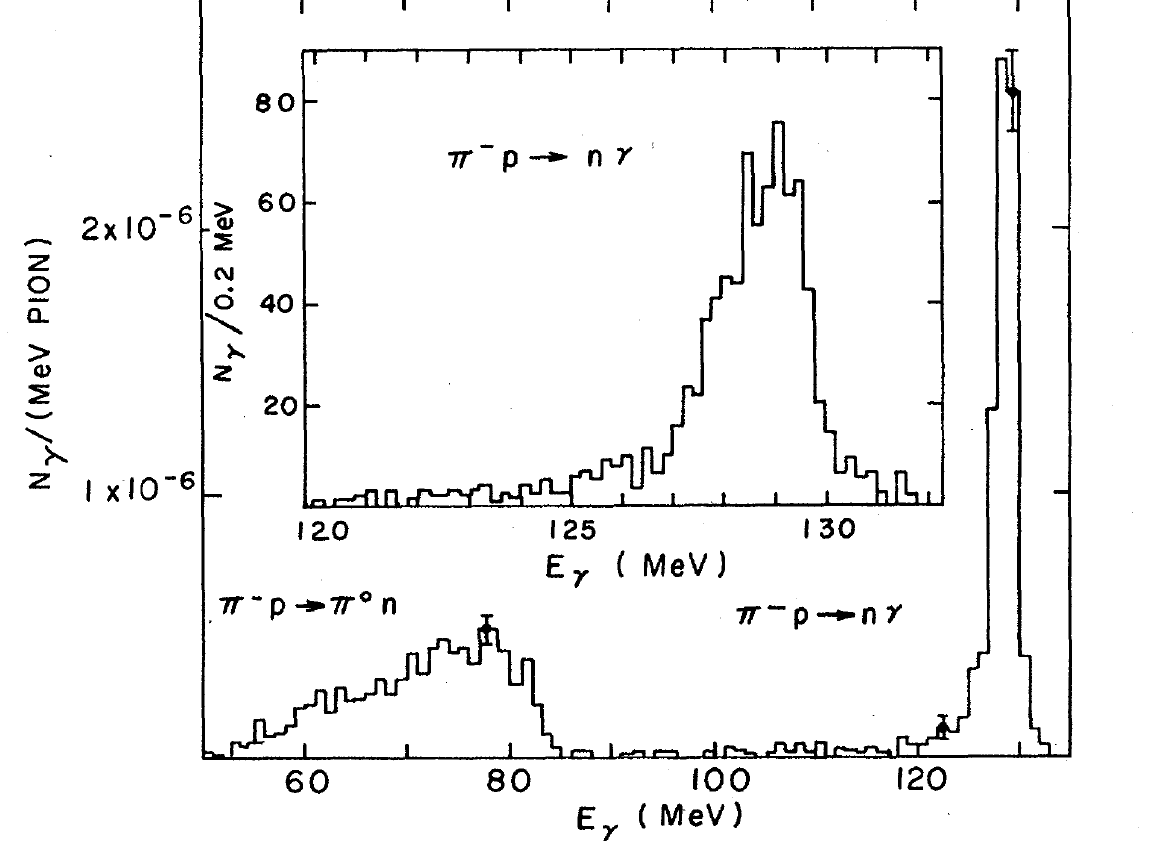
\includegraphics[width=0.9\textwidth]{png/1971_bistirlich_fig_02_h2}
  \captionsetup{width=.8\linewidth}
  \caption[width=0.9\textwidth]{
      \label{figure:1971_bistirlich_fig_02_h2}
    Photon energy spectrum from negative pion capture on hydrogen \cite{RPC_1972_Bistirlich_PhysRevC.5.1867}.
    }
 \end{minipage}
 \begin{minipage}{.5\textwidth}
  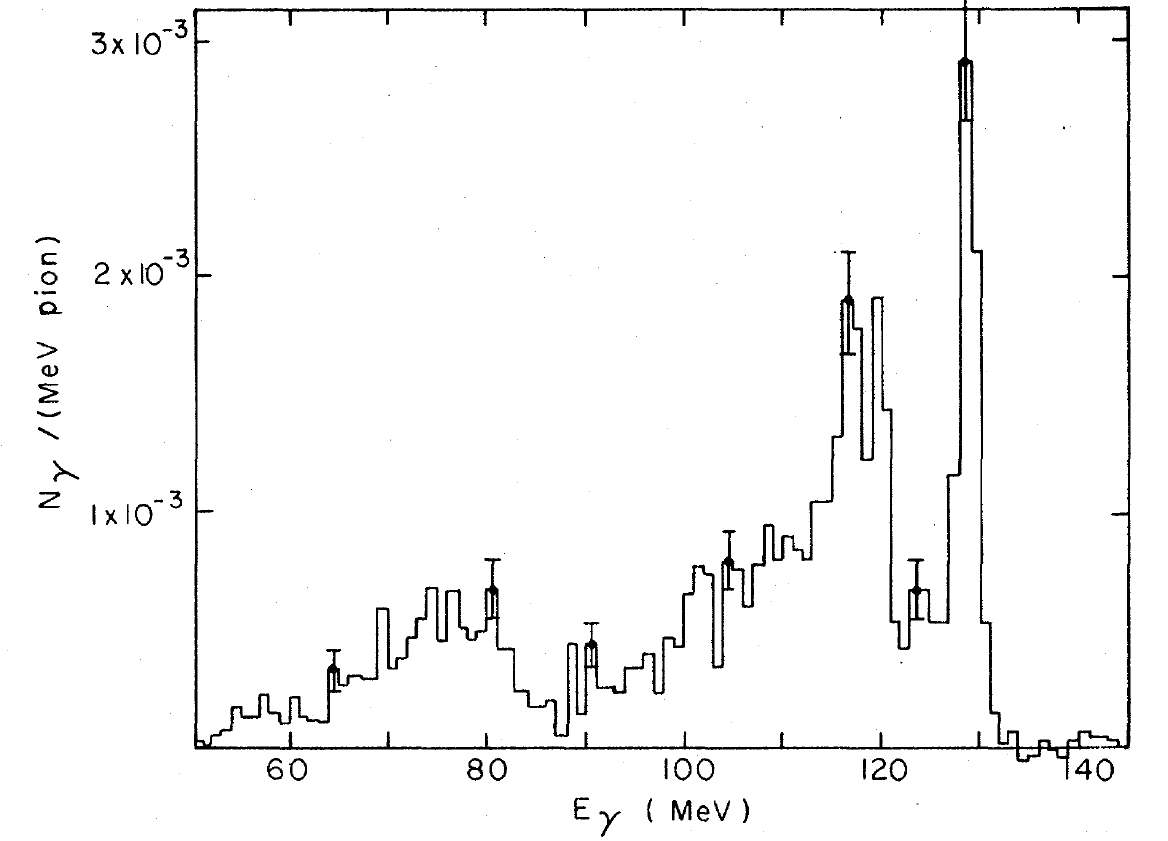
\includegraphics[width=0.9\textwidth]{png/1971_bistirlich_fig_09_ch2}
  \captionsetup{width=.8\linewidth}
  \caption[width=0.9\textwidth]{
  \label{figure:1971_bistirlich_fig_09_ch2}
    Photon energy spectrum from negative pion capture on $\rm{CH_2}$ \cite{RPC_1972_Bistirlich_PhysRevC.5.1867}.
   }
 \end{minipage}
\end{figure}

The probability of pion capture on the hydrogen component of the $\rm{CH_2}$ compound is
$\newline \rm{ W_H = (12.9 \pm 1.8) \times 10^{-3 }}$
 as used in Ref.~\cite{RPC_1991_Harston_PhysRevA.44.103}
 , an average of previous measurements. 
 This accounts for both hydrogen atoms in the $\rm{CH_2}$ molecule, and is larger than but consistent with the
 corresponding measurement (expressed as percent) in Ref.~\cite{RPC_1972_Bistirlich_PhysRevC.5.1867}.
 Negative pions captured on hydrogen have a $ (41.4 \pm 3.2) \% $
 probability of interacting via $\pi^{-} p \to n \gamma$ and producing a photon at 129.4 MeV
 \cite{RPC_1972_Bistirlich_PhysRevC.5.1867}.
 The remaining pions captured on hydrogen produce two photons via the charge exchange reaction
 $ \pi^{-} p \to n \pi^0 $ with $\pi^0  \to \gamma \gamma $,
 which results in the lower energy peak of the hydrogen spectrum. 

Together these factors yield a probability of around $ 5 \times 10^{-3} $
for obtaining 129.4 MeV RPC photons from pion capture on $\rm{CH_2}$.

%%%%%%%%%%%%%%%%%%%%%%%%%%%%%%%%%%%%%%%%%%%%%%%%%%%%%%%%%%%%%%%%%%%%%%%%%%%%%%
\subsection{$\pi^- p \to n \gamma$ photons as a calibration line }

Photons from RPC on hydrogen could be used to calibrate the Mu2e momentum scale and,
simultaneously, measure the momentum resolution.
Consider a RPC  photon converting in the detector material 
and producing an $e^+e^-$ pair. In case of a symmetric conversion, the momenta of both particles
are $\sim$ 65 MeV/c. If the conversion vertex radius is large enough, both an electron
and a positron from $\gamma \to e^+ e^-$ may produce enough hits in the tracker
so their tracks could be reconstructed and used to reconstruct the momentum of the
converted photon.

For a given photon energy $E_\gamma \leq 150$ MeV, the $\gamma \to e^+e^-$ acceptance
is maximized for photons emitted at $90^o$ with respect to the DS axis. 

The pion degrader, proposed for which with small modifications could be used
for the calibration measurement. The degrader was introduced in order to suppress
the background to \piplusenu\ from muon decays in flight \cite{MU2E_2527_PIPLUSENU},
It is a movable disk made of non-magnetic material, inserted into the beam during
the calibration runs and moved out of the beam during the regular data taking.

Making the degrader disk out of polyethylene and surrounding it, at a larger radius, 
with a thin converter foil would allow to convert photons emitted at angles close to $90^o$
with respect to the DS axis. A schematic view of the modified degrader geometry is presented in Figure~\ref{figure:degrader_geometry_v3}.

The converter foil could be supported by a light carbon foam disk mounted on the degrader.

\begin{figure}[H]
  \begin{tikzpicture}
    \node[anchor=south west,inner sep=0] at (0,-10.) {
      % \node[shift={(0 cm,0.cm)},inner sep=0,rotate={90}] at (0,0) {}
      \makebox[\textwidth][c] {
        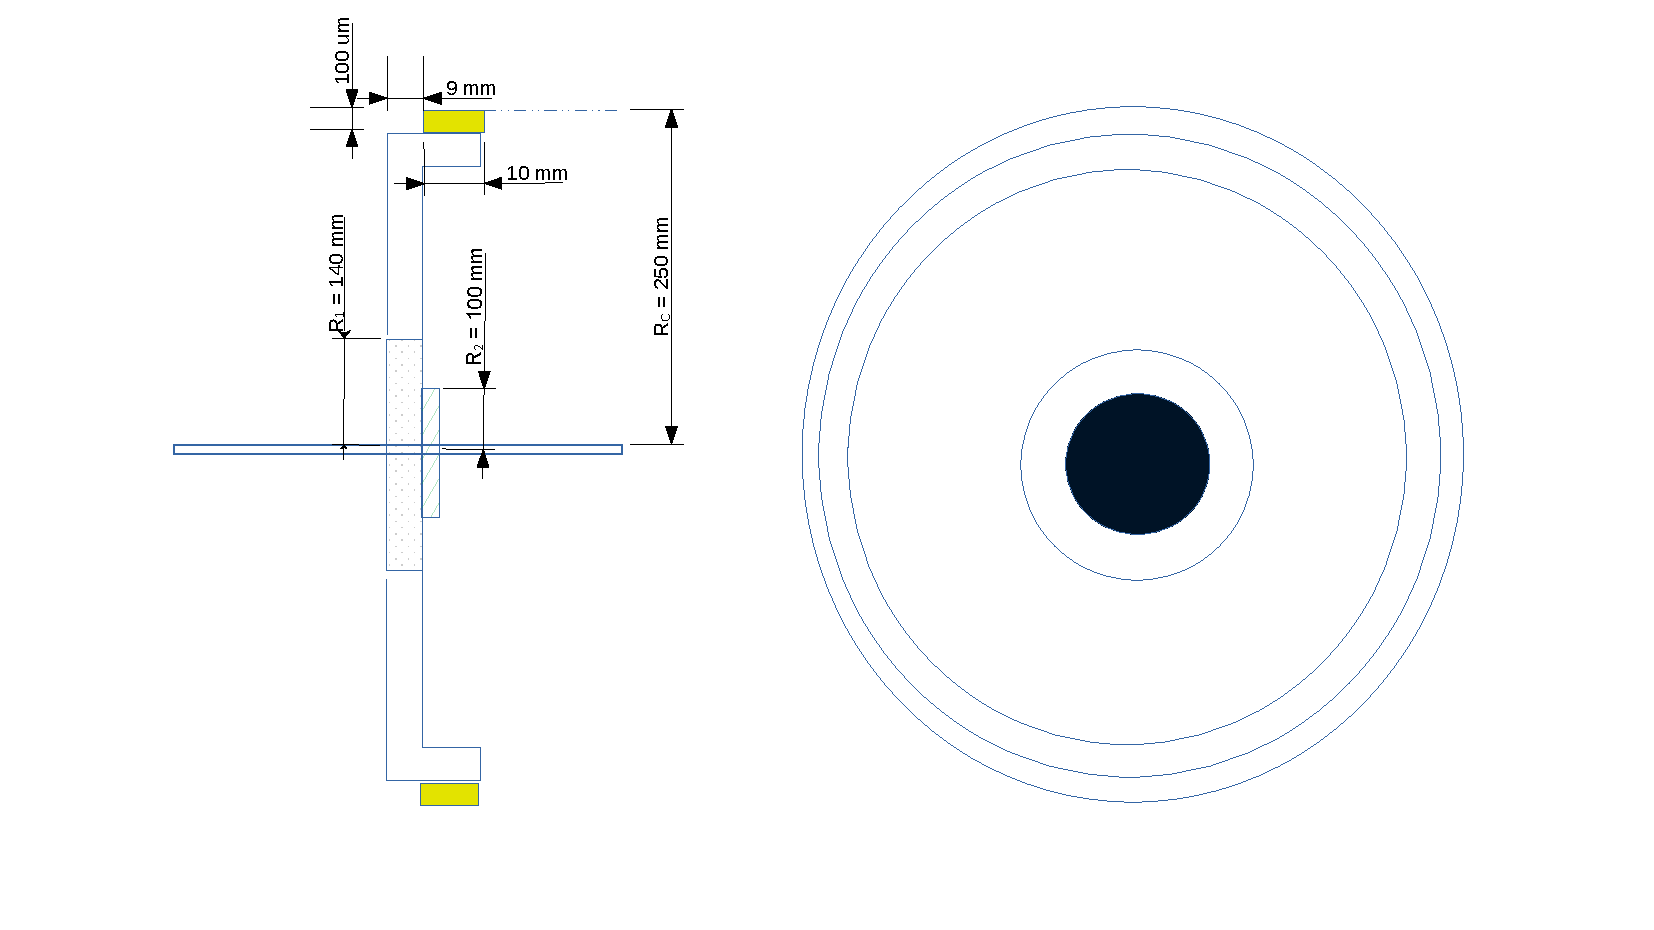
\includegraphics[width=0.95\textwidth]{pdf/degrader_geometry_002}
      }
    };
    % \node [text width=8cm, scale=1.0] at (14.5,0.5) {$\mu_B$, expected background mean};
    % \node [text width=8cm, scale=1.0, rotate={90}] at (1.5,7.5) { $S_{D}$, ``discovery'' signal strength  };
  \end{tikzpicture}
  \caption{
    \label{figure:degrader_geometry_v3}
    Schematic view of the simulated degrader geometry, not up to scale
  }
\end{figure}


%%% Local Variables:
%%% mode: latex
%%% TeX-master: t
%%% End:
